\section{Comparision}\label{sec:Comparision}

\subsection{Ballistic Deployment}

\begin{figure} \centering
  {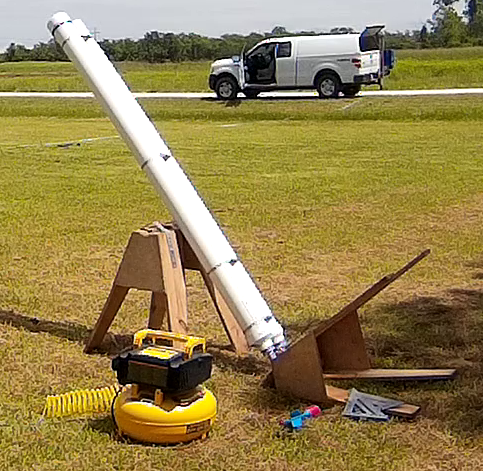
\includegraphics[width=\columnwidth]{PotatoCannon.png}}
 \caption{A pneumatic launcher for SeismicDarts.  Ballistic dart deployment has limited usefulness because the incident angle is equal to the firing angle.} 
 \label{fig:TradvsAutoDrop}
\end{figure}



\subsection{Simulation Studies}

A scheduling system to compare  time and costs for seismic surveys with varying numbers of Deployment Units, SeismicSpiders, SmartDarts, and Human manual laborers was coded in  {\sc Matlab}, available at \cite{Srikanth2016seismicScheduler}.

\begin{figure*}
\centering
\renewcommand{\figwid}{0.5\columnwidth}
\begin{overpic}[width =\figwid]{sim1_1.pdf}
\end{overpic}
\begin{overpic}[width =\figwid]{sim1_2.pdf}
\end{overpic}
\begin{overpic}[width =\figwid]{sim1_3.pdf}
\end{overpic}
\begin{overpic}[width =\figwid]{sim1_4.pdf}
\end{overpic}

\caption{Simulations were performed to estimate time take by different sensors a.) Only seismic spiders b.) Smart darts and deployment system c.) Heterogeneous System d.) Human workers
\label{fig:OneUAVsim}}
\end{figure*}
\begin{figure} \centering
  {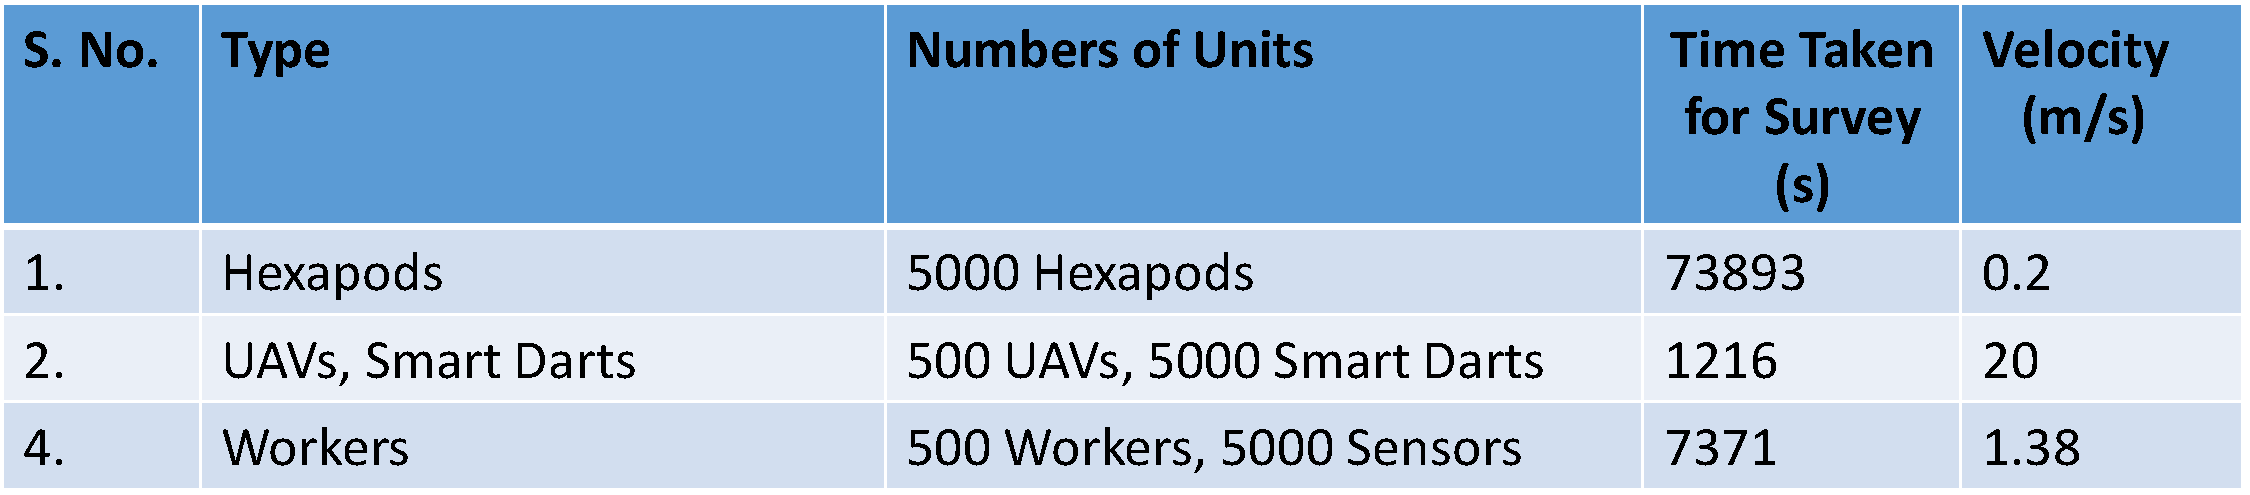
\includegraphics[width=\columnwidth]{simulation_table.pdf}}
 \caption{Simulations were performed to estimate time take by different sensors a.) Only seismic spiders b.) Smart darts and deployment system c.) Heterogeneous System d.) Human workers} 
 \label{fig:TradvsAutoDrop}
\end{figure}